\documentclass[hyperref={xetex}]{beamer}
\title{Wissenschaftliches Rechnen mit Matlab/Python}
\subtitle{Einheit1 - Einleitung, Vektoren und Matrizen}
\mode<article>
{
  \usepackage{fullpage}
  \usepackage{pgf}
  \usepackage{hyperref}
  \setjobnamebeamerversion{beamer}
}

\mode<presentation>
{
  %\usetheme{Frankfurt}
 %\usetheme{My}
  \usetheme{Madrid}
  % or ...
%\usecolortheme{seagull}
  %\setbeamercovered{transparent}
  %\setbeamercovered{dynamic}
  % or whatever (possibly just delete it)
}
\usenavigationsymbolstemplate{}
\usefonttheme{structurebold}
\usepackage{multimedia}
\usepackage{tikz}
\usepackage{fontspec,xunicode,xltxtra}
%\usepackage[scaled=.90]{helvet}
% Or whatever. Note that the encoding and the font should match. If T1
% does not look nice, try deleting the line with the fontenc.

\setbeamertemplate{footline}
{
\leavevmode
%\hbox{\begin{beamercolorbox}[wd=.5\paperwidth,ht=2.5ex,dp=1.125ex,
%leftskip=.3cm plus1fill,rightskip=.3cm]{author in head/foot}%
%    \usebeamerfont{author in head/foot}\insertshortauthor
%  \end{beamercolorbox}%
%  \begin{beamercolorbox}[wd=.5\paperwidth,ht=2.5ex,dp=1.125ex,leftskip=.3cm,
%rightskip=.3cm plus1fil]{title in head/foot}%
%    \usebeamerfont{title in head/foot}\insertshorttitle\hfill

\hfill\insertframenumber  \hspace{3pt}

%\inserttotalframenumber
%\hspace*{2ex}
%  \end{beamercolorbox}}%
  \vskip3pt%
}

%\usepackage[english]{babel}
\usepackage[ngerman]{babel}
\selectlanguage{ngerman}

%
% math/symbols
%
\usepackage{amssymb}
\usepackage{amsthm}
% \usepackage{latexsym}
\usepackage{amsmath}
%\usepackage{listings}
\usepackage[framed]{mcode}
%\usepackage{mcode}

\usepackage{mydef}
\usepackage{cmap} % you can search in the pdf for umlauts and ligatures
%\usepackage{colonequals} %corrects the definition-symbols \colonequals (besides others)
\title{Einführung in Matlab}
%
%\subtitle{Disputation} % (optional)

\author{Jochen Schulz}
% - Use the \inst{?} command only if the authors have different
%   affiliation.

\institute{Georg-August Universit\"at G\"ottingen \pgfimage[height=0.5cm]{../figures/unilogo3}}
% - Use the \inst command only if there are several affiliations.
% - Keep it simple, no one is interested in your street address.

\date{\today}

\subject{Einführung in Matlab}
% This is only inserted into the PDF information catalog. Can be left
% out. 



% If you have a file called "university-logo-filename.xxx", where xxx
% is a graphic format that can be processed by latex or pdflatex,
% resp., then you can add a logo as follows:

%\logo{\pgfimage[height=0.5cm]{figures/unilogo3}}


% Delete this, if you do not want the table of contents to pop up at
% the beginning of each subsection:
% \AtBeginSubsection[]
% {
%   \begin{frame}<beamer>
%     \frametitle{Aufbau}
%     \tableofcontents[currentsection,currentsubsection]
%   \end{frame}
% }

\AtBeginSection[]
{
  \begin{frame}<beamer>
    \frametitle{Aufbau}
    \tableofcontents[currentsection,currentsubsection]
  \end{frame}
}


\begin{document}



\begin{document}
\titlepage


\begin{frame}{Organisatorisches}
\begin{itemize}
\item Anmeldung $\rightarrow$ StudIP \\
      \url{https://studip.uni-goettingen.de/}

{\color{blue}{Wissenschaftliches Rechnen mit Matlab/Python (Mathematische Anwendersysteme)}}
\item Alle Unterlagen (Aufgabenblätter, Vorlesungsfolien, Beispiele, Musterlösungen) $\rightarrow$ StudIP
\pause
\begin{block}{Dozent}
Jochen Schulz\\
NAM, Zimmer 04 (Erdgescho{\ss})\\
\textbf{Telefon}: 39-4525\\
\textbf{Email}: \href{mailto:schulz@math.uni-goettingen.de}{\texttt{schulz@math.uni-goettingen.de}}\\
\textbf{XMPP}: \url{jschulz1@jabber.gwdg.de}\\

\end{block}
\end{itemize}
\end{frame}


\begin{frame}{Ablauf der Veranstaltung}
\begin{itemize}
\item Blockveranstaltung vom  22.9 - 10.10.2014
\item \alert{Vorlesung:} 9.15 - ca. 11.30  (MN55)
\item \alert{Übungsbetrieb/Praktikum}: ca. 11:30 - ca. 17:00  (MultimediaRaum MI)
\begin{itemize}
\item 1 Übungszettel/Tag.
\item Besprechung Aufgaben vom Vortag (individuell)
\item Betreuung: Hilfestellung beim Bearbeiten der Aufgaben
%\item Klausurzulassung: 3 beliebige markierte Aufgaben/Woche testieren lassen. 
\end{itemize}
\item \alert{Klausur:} 10.10.2014; 13:00 - 14:30
\end{itemize}

\end{frame}

\begin{frame}{Inhalt der Vorlesung}
\begin{description}
\item[1. Tag] Organisatorisches, Basis von Matlab und Python
\item [2. Tag] Programmieren, Datenstrukturen
\item [3. Tag] Rekursionen, Grafik
\item [4. Tag] ? Polynome, Interpolation, Debugging
\item [5. Tag] ? Mehrdimensionale Arrays, Funktionen, Numerische Lineare Algebra, Dünnbesetzte Matrizen
\item [6. Tag] ? Numerische Mathematik, Profiler
\item [7. Tag] ? Visualisierung und Validierung
\item [8. Tag] ? Schnittstelle zu C (Optional)
\item [9. Tag] ? Wunschvorlesung
\item [10. Tag] Fragestunde
\end{description}
\end{frame}

\begin{frame}{Aufbau}
\tableofcontents
\end{frame}

\section{MATLAB und Python Basis}

\subsection{Einleitung}

\begin{frame}{Programmieren für den Wissenschaftler}
  \begin{itemize}
    \item Daten erzeugen oder erheben (Simulation, Experiment)
    \item Weiterverarbeitung von Daten
    \item Visualisierung und Validierung
    \item Ergebnisse veröffentlichen bzw. kommunizieren
  \end{itemize}

  \begin{block}{}
Wir wollen: eine \emph{High-Level} Sprache:
\begin{itemize}
\item Programmieren ist leicht
\item Vorhandene Elemente nutzen
\item geeignet für Prototyping und Debugging (Interaktion)
\item Möglichst nur ein Werkzeug für alle Probleme
\end{itemize}
\end{block}

\end{frame}

%-------------------------------------------------
%  Folie:
%-------------------------------------------------
\begin{frame}[fragile]{MATLAB}

\begin{itemize}
\item MATLAB steht für \alert{Mat}rix \alert{lab}oratory; ursprünglich speziell Matrizenrechnung.
\item Interaktives System für numerische Berechnungen und Visualisierungen (Skriptsprache).
\end{itemize}
\begin{block}{Vorteile}
\begin{itemize}
\item Vielfältige Visualisierungsmöglichkeiten.
\item Viele zusätzliche Toolboxes (Symb. Math T., PDE T., Wavelet T.)  
\item Ausgereifte und integrierte Oberfläche.
\end{itemize}
\end{block}
\begin{block}{Nachteile}
    \begin{itemize}
        \item Kostenintensiv.
        \item Ein/Ausgabe von Dateien kann umständlich sein.
        \item Spezialisierter Funktionsumfang macht manche Programmierung schwer.
    \end{itemize}
  
\end{block}
\end{frame}

\begin{frame}[fragile]{Python: NumPy, SciPy, SymPy}

\begin{itemize}
  \item Modulare Skriptsprache.
\end{itemize}

\begin{block}{Vorteile}
\begin{itemize}
  \item Viele Module mit wissenschaftlichen Fokus.
  \item Klare Code-Struktur.
  \item Ebenso viele Module für den nicht-wissenschaftlichen Gebrauch (nützlich z.B. für Ein-/Ausgabe).
  \item Frei und open-source.
\end{itemize}
  
\end{block}
\begin{block}{Nachteile}
\begin{itemize}
  \item Entwicklungsumgebung etwas komplizierter (Spyder,ipython).
  \item Nicht alle spezialisierten Möglichkeiten anderer Software.
\end{itemize}
  
\end{block}
\end{frame}


%-------------------------------------------------
%  Folie:
%-------------------------------------------------
\begin{frame}[fragile]{Literatur}
  \begin{block}{MATLAB}
  \begin{thebibliography}{10}
\small
\bibitem{1} \alert{Matlab online-help :-)}.
\bibitem{3} \alert{Introduction to Scientific Computing}, C.F. van Loan, Prentice Hall,
New Jersey, 1997,
\bibitem{4} \alert{Scientific Computing with MATLAB}, A. Quarteroni, F. Saleri, Springer, 2003,
\end{thebibliography}
\end{block}
\begin{block}{Python}
  \begin{thebibliography}{10}
      \small
    \bibitem{1} \alert{NumPy, SciPy} SciPy developers (\url{http://scipy.org/}),
    \bibitem{2} \alert{SciPy-lectures}, F. Perez, E. Gouillart, G. Varoquaux, V. Haenel (\url{http://scipy-lectures.github.io}),
    \bibitem{3} \alert{Matplotlib} (\url{http://matplotlib.org})
    \bibitem{4} \alert{scitools} (\url{https://code.google.com/p/scitools/}) 
    \bibitem{5} \alert{mayavi} (\url{http://docs.enthought.com/mayavi/mayavi/mlab.html})
  \end{thebibliography}
\end{block}
\end{frame}


\subsection{Grundlegende Bedienung MATLAB}
%-------------------------------------------------
%  Folie:
%-------------------------------------------------
\begin{frame}[fragile]{MATLAB Fenster-Aufbau}
Starten von MATLAB: Eingabe von \mcode{matlab &} (in einem Terminal).
\centering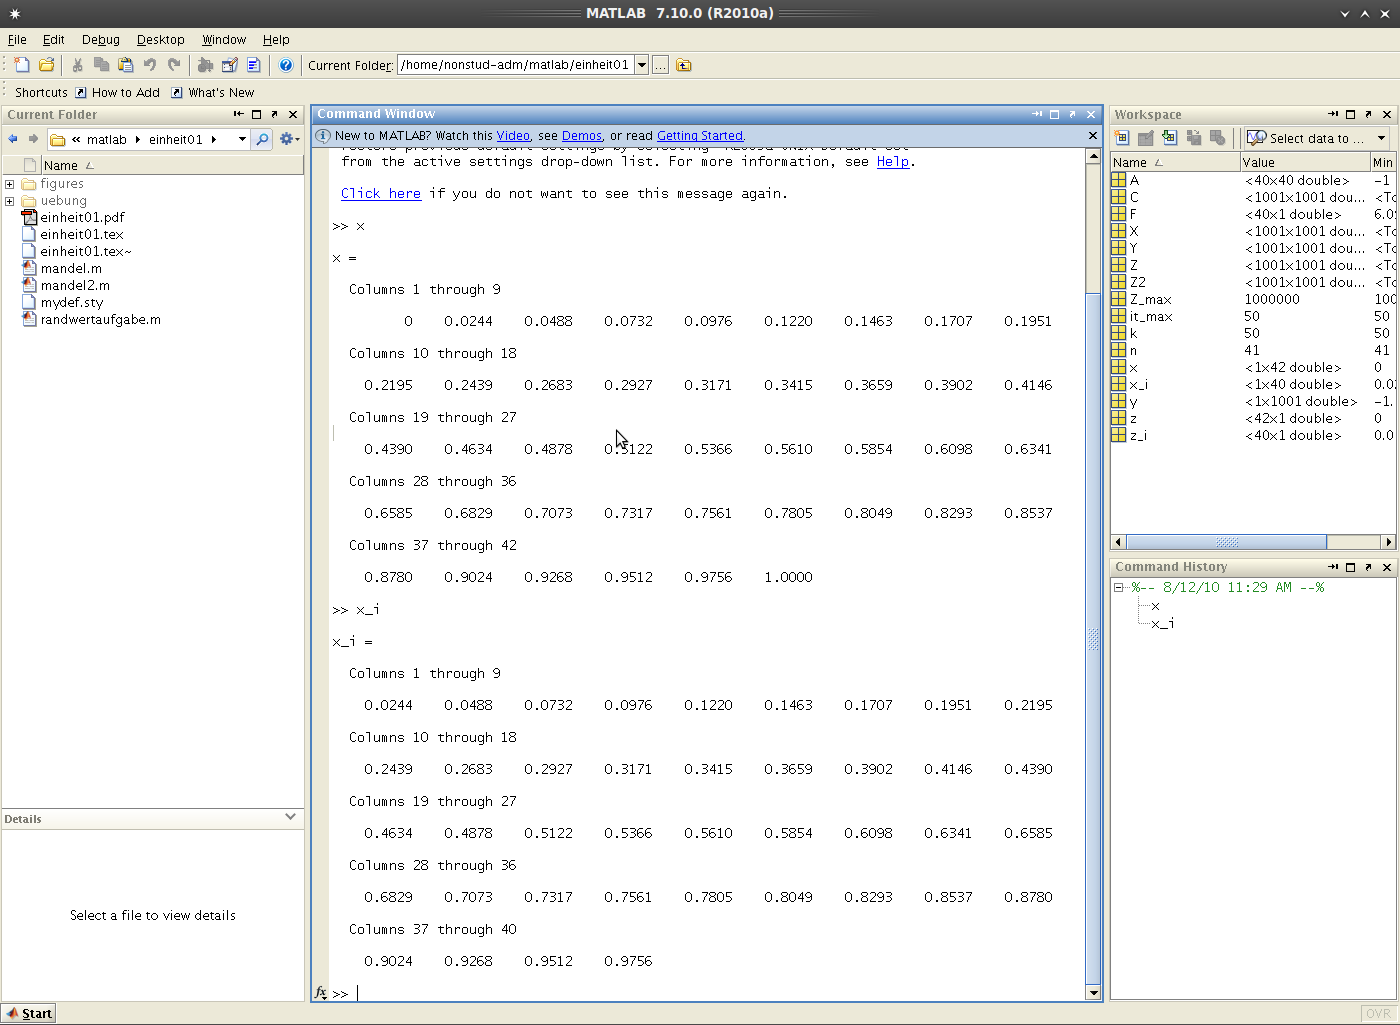
\includegraphics[width=1\textwidth]{figures/Screenshot-MATLAB}

\end{frame}

%basis-Befehlsreferenz? clear? pfeiltasten etc. Kommentare?
% vor ort zeigen

%-------------------------------------------------
%  Folie:
%-------------------------------------------------
%\begin{frame}[fragile]{Workspace - globale Variablen}
%\begin{itemize}
%\item Alle definierten (globalen) Variablen werden im Workspace gespeichert.
%\item Zugriff während einer MATLAB-Sitzung.
%\item Inhalt des Arbeitsspeichers: \mcode{whos} oder \mcode{who}
%\begin{matlabin}
%>> whos
%  Name      Size            Bytes  Class   
%
%  ans       1x1                 8  double    
%\end{matlabin}
%\item Löschen von Variablen : \mcode{clear <var>};\\
%\mcode{clear} löscht den gesamten Arbeitsspeicher (Workspace).
%\end{itemize}
%\end{frame}



%\subsection{Programm-Dateien und der Editor}


%----------------------------
% Folie 
%----------------------------
\begin{frame}[fragile]{Struktur von Skript-Files}
\begin{itemize}
\item Skript-Files bestehen aus einer Sequenz von Befehlen, die
  nacheinander abgearbeitet werden (imperatives Programmierparadgima)

\item operiert auf Variablen im \textit{Workspace}.

\item Gestartet wird das Programm \mcode{name.m} durch Eingabe von
  \mcode{name}.

\item Beschreibung des Skript-Files (oder der Funktion):
\begin{matlabin}
help sin
\end{matlabin}
\begin{matlab}
   sin    Sine of argument in radians.
      sin(X) is the sine of the elements of X.
\end{matlab}


\end{itemize}
\end{frame}

%----------------------------
% Folie 
%----------------------------
\begin{frame}[fragile]{Struktur von Function-Files}
\begin{matlabin}
function [Out_1,..,Out_k] = myfunction(In_1,..,In_l)
% Beschreibung der Funktion
 ..
Out_1=..
 ..
Out_k=..
\end{matlabin}
Soll keine Variable zurückgegeben werden, so besteht die erste Zeile aus
\begin{matlabin}
function myfunction(In_1,..,In_k)
\end{matlabin}
\begin{itemize}
\item Call-by-value (Argumente werden im Speicher kopiert)

\item Variablen lokal, d.h.
\begin{itemize}
 \item Variablen des Workspace sind  nicht verfügbar.
\item definierte Variablen werden nicht im  Workspace gespeichert.
\end{itemize}
\end{itemize}
\alert{Wichtig:} Funktionsname = Dateiname.
\end{frame}

%----------------------------
% Folie 
%----------------------------
\begin{frame}[fragile]{Priorität beim Programmaufruf}
Beispiel-Programmaufruf
\begin{matlabin}
name
\end{matlabin}

Testet ob,..
\begin{enumerate}
\item  \alert{Variable}
\item  \alert{Unterfunktion}. Eine
  Unterfunktion ist ein Programm/Funktion, die in derselben Datei wie der
  Aufruf steht.
\item  Programm im \alert{aktuellen Verzeichnis}.
\item  \textit{private function}.
\item  Programm im \alert{Suchpfad}. 
\end{enumerate}
Bei gefundenem Namen wird die Suche beendet.
\end{frame}

%----------------------------
% Folie 
%----------------------------
\begin{frame}[fragile]{Suchpfad}

Der Suchpfad (Variable \mcode{path}) enthält Verzeichnisse in einer geordneten Liste.

\begin{itemize}
\item Abarbeitung erfolgt der Ordnung gemäss.
\item  Suchpfade hinzufügen:
\begin{matlabin}
addpath <pfadname>
\end{matlabin}
\item Suchpfade entfernen:
\begin{matlabin}
rmpath <pfadname>
\end{matlabin}
\end{itemize}
\end{frame}


%----------------------------
% Folie 
%----------------------------
\begin{frame}[fragile]{Bedienung: Kurzreferenz}
\begin{itemize}
\item \alert{ \mcode{doc <name>}}\\ öffnet grafisches Hilfefenster zum jeweiligen Programm.
  \item \alert{F5}\\ führt offene Datei im command window aus.
  \item \alert{F9}\\ führt markierte Code-Zeilen aus.
  \item \alert{clear}\\ löscht Variablen im Workspace
\item \alert{ \mcode{lookfor <name>}} \\ Suche nach \mcode{name} in den
  Kommentaren zu den Funktionen (auch: grafisches Hilfefenster).
\item  \alert{ \mcode{what}}\\ m-Files im aktuellen Verzeichnis.
\item  \alert{ \mcode{type <name>}}\\ Inhalt von \mcode{name.m} (Command Window).
\item  \alert{ \mcode{which <name>}}\\ absoluter Pfad der Datei, in dem die  Funktion
  \mcode{name} gespeichert ist. 
\end{itemize}
\end{frame}


\subsection{Grundlegende Bedienung Python (Spyder)}


\begin{frame}[fragile]{Spyder Fenster-Aufbau}
Starten von Spyder: Eingabe von \mcode{spyder &} (in einem Terminal).
\centering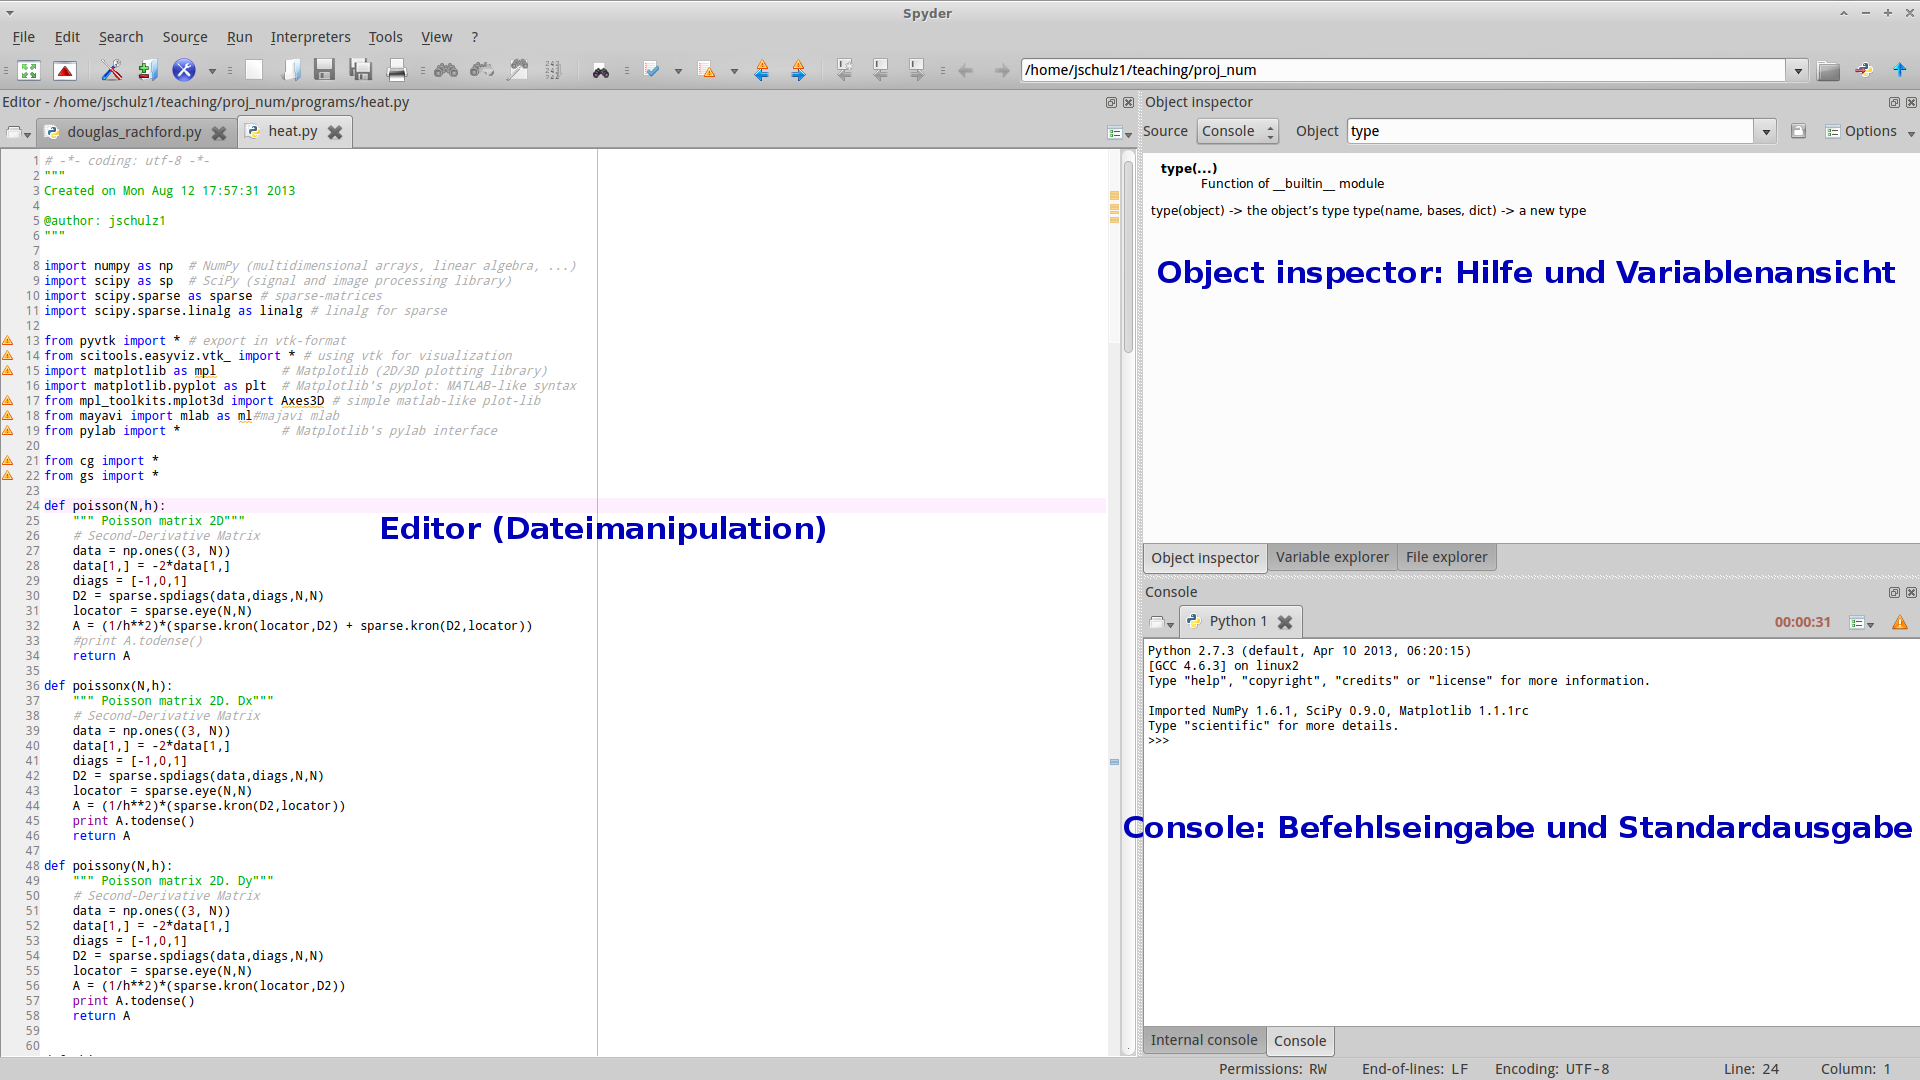
\includegraphics[width=1\textwidth]{figures/Screenshot_spyder}

\end{frame}

\begin{frame}[fragile]{Struktur von Skript-Files}
\begin{itemize}
\item Skript-Files bestehen aus einer Sequenz von Befehlen, die
  nacheinander abgearbeitet werden, sowie von definierten Funktionen
\item enthält geladene Module.
\item operiert auf globalen Variablen.

\item Gestartet wird das Programm \isage{name.py} durch F5 im Editor oder in einem terminal.

\end{itemize}
\end{frame}

\begin{frame}[fragile]{Funktionen}
Eine Funktion kann man wie folgt definieren:
\begin{pyin}
def <name>(<Argumente>) : 
    """ Beschreibung """
    <Code Block>
    return <Rueckgabe>
\end{pyin}
\begin{itemize}
\item Variablen lokal.
\item \textsl{Call-by-reference} (Referenz zum Objekt wird übergeben)
\item \alert{Objekt-Methoden}:\\
  \begin{itemize}
    \item Objekte besitzen Funktionen, sogenannte Objekt-Methoden.
\item Ein Objekt kennt alle auf sich selbst anwendbaren Funktionen.
  \end{itemize}

\begin{pyin}
f = 3.14
f.is_integer()
\end{pyin}
\end{itemize}

\end{frame}


\begin{frame}[fragile]{Priorität beim Programmaufruf}

Beispiel-Programmaufruf
\begin{pyin}
name
\end{pyin}

Testet ob,..
\begin{enumerate}
\item  \alert{Variable}
\item  \alert{Funktion/Objekt} 
\end{enumerate}
Bei gefundenem Namen wird die Suche beendet.
\end{frame}


\begin{frame}{Bedienung : Kurzreferenz}
  Programm:  spyder 
\begin{itemize}
\item \alert{ \isage{<name>?}}\\ öffnet Hilfe zur jeweiligen Funktion.
\item \alert{F5}\\ führt offene Datei in dedizierter oder vorhandener Shell aus.
\item \alert{F9}\\ führt markierte Code-Zeilen aus.
\item \alert{\isage{<name>.TAB}} \\ zeigt alle Objektmethoden.
\end{itemize}
\end{frame}

\subsection{Erstes Beispiel}
%----------------------------
% Folie 
%----------------------------
\begin{frame}[fragile]{Graph eines Polynoms}

\alert{Aufgabe:}\\
Zeichnen Sie  den Graphen eines Polynoms
\vspace*{-0.4cm}
\[ p(x)= \sum_{i=0}^N a_i x^i, \quad a_i \in \mathbb{R} 
\vspace*{-0.4cm} \]
Zu Werten $(x_i)_{i=1}^n$ muß man $(p(x_i))_{i=1}^n$ berechnen.

\end{frame}

%----------------------------
% Folie 
%----------------------------
\begin{frame}[fragile]{Skalare Version}
\begin{matlabin}[title=\tiny matlab]
function y=ausw_poly1(a,x)

n = length(a);
aux_vector = x.^(0:n-1);
y = aux_vector*transpose(a);
\end{matlabin}
\begin{pyin}[title=\tiny python]
def ausw_poly1(a,x):
    n = len(a)
    aux_vector = x**np.array(range(0,n))
    return dot(aux_vector,a)
\end{pyin}


\end{frame}
%----------------------------
% Folie 
%----------------------------
\begin{frame}[fragile]{Vektorielle Version}
\begin{matlabin}[title=\tiny matlab]
function y = ausw_poly2(a,x)
n = length(a);
k = length(x);
A = repmat(transpose(x),1,n);
B = repmat(0:(n-1),k,1);
y = (A.^B)*transpose(a);
\end{matlabin}
\begin{pyin}[title=\tiny python]
def ausw_poly2(a,x):
    n = len(a)
    k = len(x)
    xm = np.array([x])
    A = sp.repeat(xm.T, n,1)
    B = sp.repeat(np.array([range(0,n)]), k,0)
    return dot(A**B,a)
\end{pyin}
\end{frame}
%----------------------------
% Folie 
%----------------------------
\begin{frame}[fragile]{Plotten des Polynoms}
\begin{matlabin}[title=\tiny matlab]
a = [9 0 -10 0 1]; % Koeffizienten

x = linspace(0,4,30); % Betrachte [0,4]
y = ausw_poly2(a,x);
% Plotten
plot(x,y,'r*-','LineWidth',3,'MarkerSize',4)
\end{matlabin}
\begin{pyin}[title=\tiny python]
a = np.array([9,0,-10,0,1])

x = np.linspace(0,4,30) # Betrachte [0,4]
y = ausw_poly2(a,x)
#Plotten
plot(x,y,'r*-',linewidth=3,markersize=8)
\end{pyin}
\end{frame}
%----------------------------
% Folie 
%----------------------------
\begin{frame}[fragile]{Plotten des Polynoms}
\begin{center}
\begin{columns}[c]
\column{0.48\textwidth}
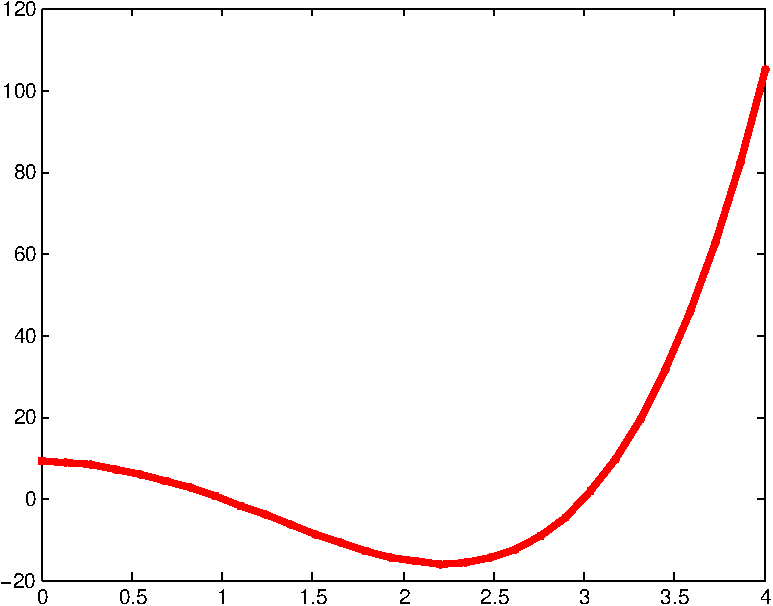
\includegraphics[width=0.8\textwidth]{figures/polynom_ma} 

\centerline{Matlab}
\column{0.48\textwidth}
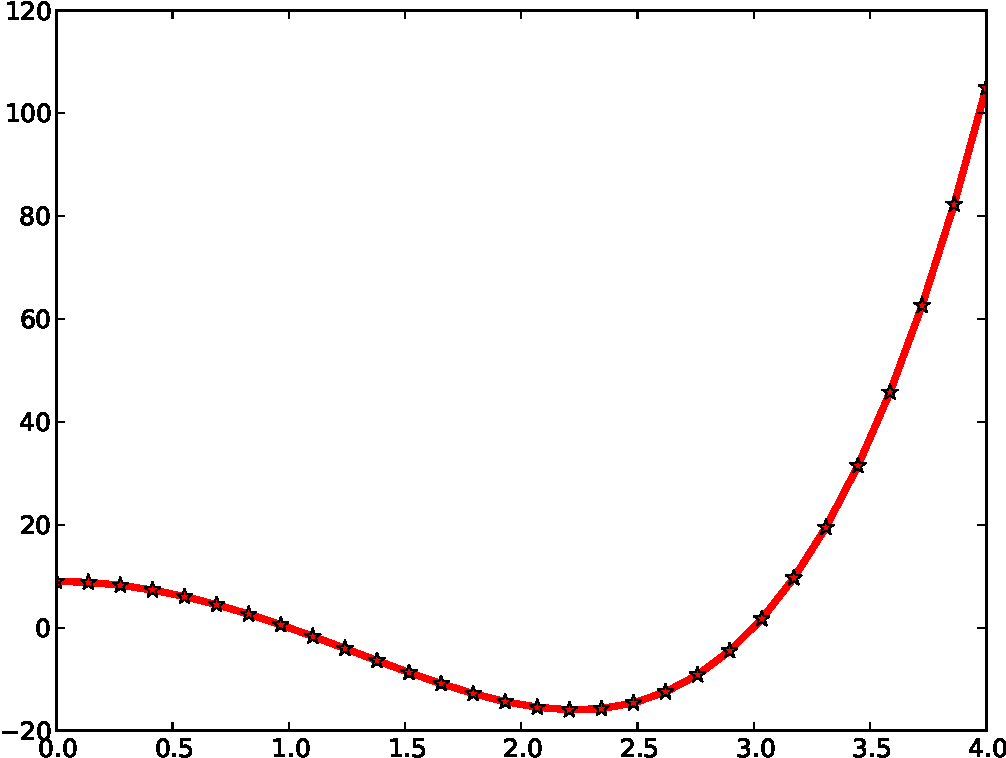
\includegraphics[width=0.8\textwidth]{figures/polynom_py} 

\centerline{Python}
\end{columns}
\end{center}

\end{frame}

\section{Programmieren: Basis}

\begin{frame}[fragile]{Bezeichner}
\begin{itemize}
\item \alert{Bezeichner} sind Namen, wie z.B. $x$ oder $f$. Sie können
im mathematischen Kontext sowohl Variablen als auch Unbestimmte repräsentieren.
\item Bezeichner sind aus Buchstaben, Ziffern und
Unterstrich \_ zusammengesetzt.
\item Man unterscheidet zwischen Groß- und Kleinschreibung.
\item Bezeichner dürfen nicht mit einer Ziffer beginnen.
\end{itemize}
\textbf{Beispiele}
\begin{itemize}
\item zulässige Bezeichner:
\isage{x}, \isage{f}, \isage{x23}, \isage{_x_1}
\item unzulässige Bezeichner:
\isage{12x}, \isage{p~}, \isage{x>y}, \isage{Das System}
\end{itemize}
\end{frame}

\begin{frame}[fragile]{Typen und Werte eines Bezeichners}
\begin{itemize}
\item \alert{Datentyp}: Eigenschaften der Daten. \\
  \textbf{Beispiel}: ganze Zahlen, Zeichenketten, Gleitkommazahlen, Listen  \ldots  
  \begin{itemize}
    \item Matlab: 2D-Arrays vom Typ \mcode{Double} vorherrschend
    \item Python: \isage{integer}, \isage{float}, \isage{numpy.ndarray}, \isage{list},..
  \end{itemize}
\item \alert{Objekt}: Instanz (Einheit) eines Datentyps.
\item \alert{Wert} eines Bezeichners: ein \alert{Objekt} eines bestimmten
\alert{Datentyps}.
\end{itemize}
\end{frame}

\begin{frame}[fragile]{Zuweisungsoperator $=$}
    \begin{pyin}
<bezeichner> = <wert>
    \end{pyin}   
Zuweisung des Wertes \isage{wert} zu dem Bezeichner \isage{bezeichner}. Dabei wird der Typ automatisch festgelegt.
\begin{itemize}
\item \textbf{Warnung:} Unterscheiden Sie  stets zwischen dem Zuweisungsoperator {\color{blue} $=$} und
dem logischen Operator {\color{blue} $==$}.   
\item Löschen von Zuweisungen/Variablen.
\begin{itemize}
\item Python: {\color{blue} \isage{\%clear <bezeichner>}}
\item Matlab: {\color{blue} \isage{clear <bezeichner>}}
\end{itemize}
\end{itemize}

\textsl{Beispiel}:

\begin{pyin}
  a = 5.5
  type (a)
\end{pyin}
\begin{pyout}
  float
\end{pyout}

%\item {\color{blue} \isage{func(arg)=expr(arg)}}: Definition der Funktion \isage{func} mit dem Argument \isage{arg} und Zuweisung des Ausdrucks \isage{expr} zu (abhängig von \isage{arg})
%%\item Rückgabeparameter ist die rechte Seite (Eine Ausgabe erfolgt jedoch normalerweise nicht)
\end{frame}

\begin{frame}[fragile]{Python: Listen und Tuple}
 \begin{itemize}
\item Eine \alert{Liste} ist in Python mit \isage{[..,..]} gekennzeichnet (hat Ordnung, veränderbar (mutable)) 
\begin{pyin}
liste = [21,22,24,23]
liste.sort(); liste 
\end{pyin}
\begin{pyout}
 [21, 22, 23, 24]
\end{pyout}
\item Ein \alert{Tuple} ist in Python mit \isage{(..,..)} gekennzeichnet (hat Struktur, nicht veränderbar (immutable))
\begin{pyin}
tuple = (liste[0], liste[2])
tuple, tuple[0]
\end{pyin}
\begin{pyout}
(( 21, 24), 21) 
\end{pyout}
 \end{itemize}
\end{frame}


\section{Vektoren und Matrizen}



\subsection{Erzeugen von Vektoren}
%
% Slide: 
%
\begin{frame}[fragile]{}
\begin{itemize}
\item Erzeugen 'per Hand'
\begin{matlabin}
b = [1 2 4]
\end{matlabin}
\begin{pyin}
b = np.array([1,2,4])
\end{pyin}

\item Abfragen der Einträge von $b$
\begin{matlabin}
b(2)
\end{matlabin}
\begin{pyin}
b[1]
\end{pyin}

Index $\equiv$ Position im Vektor\\

\alert{Achtung}: 

\begin{itemize}
  \item \emph{Matlab}: Indizes beginnen immer mit $1$!
\item \emph{Python}: Indizes beginnen immer mit $0$!
\end{itemize}

\end{itemize}
\end{frame}

%
% Slide: 
\begin{frame}[fragile]{Matlab: Doppelpunkt - Notation}
\mcode{x:s:z} erzeugt einen Vektor der Form 
\[ (x,x+s,x+2s,x+3s, \ldots ,z). \]
$x + ns \leq z$ für alle $n$. 
Schrittweite $s$ ist 1 wenn nur ein Doppelpunkt benutzt wird.
\begin{matlabin}
>> a = 2:11
a =
 2  3  4  5  6  7  8  9  10  11

>> c = -2:0.75:1
c =
 -2.0000 -1.2500 -0.5000 0.2500 1.0000
\end{matlabin}
\end{frame} 

\begin{frame}[fragile]{Python: ogrid-Slicing}
\isage{ogrid[x:s:z]} erzeugt einen Vektor der Form 
\[ (x,x+s,x+2s,x+3s, \ldots , z). \]
$x + ns \le z$ für alle $n$.
Schrittweite $s$ ist 1 wenn nur ein Doppelpunkt benutzt wird.
\begin{pyin}
>>> a = ogrid[2:12]
array([ 2,  3,  4,  5,  6,  7,  8,  9, 10, 11])

>>> c = ogrid[-2:1.1:0.75]
array([-2.  , -1.25, -0.5 ,  0.25,  1.  ])

\end{pyin}
\end{frame} 

%
% Slide: 
%
\begin{frame}[fragile]{}
\begin{itemize}
\item \mcode{length(a)}(Matlab) \isage{len(a)}(Python)\\ Länge des Vektors $a$ an.
\item \isage{linspace(x1,x2,N)} oder \isage{ogrid[x1:x2:Nj]}\\ Vektor
\[ x1, x1+\frac{x2-x1}{N-1}, x1+2 \frac{x2-x1}{N-1}, \dots ,x2  \]
der Länge $N$.
\begin{pyin}
linspace(1,2,4)
\end{pyin}
\begin{pyout}
array([ 1.  ,  1.33333333,  1.66666667,  2. ])
\end{pyout}

\item \mcode{logspace(x1,x2,N)}\\ wie \mcode{linspace}, nur logarith. Skalierung
\end{itemize}
\end{frame}

\subsection{Erzeugen von Matrizen}
%
% Slide: 
%
\begin{frame}[fragile]{}
\begin{itemize}
\item Erzeugen 'per Hand'
\begin{matlabin}
B = [1 3 4; 5 6 7]
\end{matlabin}
\begin{pyin}
B = np.array([[1,3,4],[5,6,7]])
#alternativ (Unterschiedlicher Datentyp!)
B = matrix([[1,3,4],[5,6,7]]) 
\end{pyin}

\item \mcode{eye(n,m)}\\ $(n \times m)$-EinheitsMatrix)
\begin{matlabin}
eye(2,3)
\end{matlabin}
\begin{matlab}
ans =
     1     0     0
     0     1     0 
\end{matlab}

($1$ auf der Hauptdiagonalen und 0 sonst).
\end{itemize}
\end{frame} 
%
% Slide: 
%
\begin{frame}[fragile]{}
\begin{itemize}
\item \mcode{zeros(n,m)}(Matlab) \isage{zeros((n,m))}(Python) \\$(n \times m)$- Matrix mit $0$ als Einträge.
\item \mcode{ones(n,m)}(Matlab) \isage{ones((n,m))}(Python)\\$(n \times m)$- Matrix mit $1$ als Einträge.
\item Blockmatrizen
\begin{matlabin}
C = [B zeros(2,2); eye(2,3) eye(2,2)]
\end{matlabin}
\begin{pyin}
C = vstack([hstack([B, zeros((2,2))] ) ,hstack([eye(2,3), eye(2,2)]) ])
\end{pyin}
\begin{matlab}
C =
     1     3     4     0     0
     5     6     7     0     0
     1     0     0     1     0
     0     1     0     0     1 
\end{matlab}

\alert{Achtung:} Matrizen in einer Zeile müssen dieselbe
Zeilenanzahl haben und Matrizen in einer Spalte dieselbe Spaltenanzahl.
\end{itemize}
\end{frame} 
%
% Slide: 
%
\begin{frame}[fragile]{}
\begin{itemize}
\item \mcode{repmat(A,n,m)}(Matlab) \isage{tile(A,(n,m)}(Python)\\ Blockmatrix mit $(n \times m)$
  aus A bestehenden Blöcken zusammenhängen
\begin{matlabin}
D = repmat(B,1,2) 
\end{matlabin}
\begin{pyin}
D = tile(B,(1,2))
\end{pyin}
\begin{matlab}
D =
     1     3     4     1     3     4
     5     6     7     5     6     7 
\end{matlab}


%\item \mcode{blkdiag(A,B)}\\ Blockdiagonalmatrix.
\item \mcode{diag(v,k)} \\Matrix der Größe $(n+|k|) \times
  (n+|k|)$ mit den Einträgen des Vektors $v$ (Länge $n$) auf der $k$-ten Nebendiagonalen. 
\end{itemize}
\end{frame}
%
% Slide: 
%
\begin{frame}[fragile]{Beispiel- und Spezial-Matrizen}
\begin{itemize}
\item Beispiel
\begin{matlabin}
E = vander(linspace(1,3,3))
\end{matlabin}
\begin{matlab}
E =
     1     1     1
     4     2     1
     9     3     1
\end{matlab}

\item Hilbert-Matrix: 
  \begin{itemize}
    \item \mcode{hilb}(Matlab) 
    \item \isage{scipy.linalg.hilbert}(Python)
  \end{itemize}
\item Hadamard-Matrix:
  \begin{itemize}
    \item \mcode{hadamard} (Matlab) 
    \item \isage{scipy.linalg.hadamard}(Python)
  \end{itemize}
\end{itemize}
\end{frame}

\subsection{Zugriff und Manipulation von Matrizen}
%
% Slide: 
%
\begin{frame}[fragile]{Matlab: Zugriff auf Matrizen}
\begin{columns}[c]%
\column{0.45\textwidth}%
\begin{matlabin}[basicstyle=\tiny]
A = [1 2 3; 4 5 6; 7 8 9]
\end{matlabin}%
\begin{matlab}
A =
     1     2     3
     4     5     6
     7     8     9 
\end{matlab}%
\end{columns}%
\begin{columns}[t,onlytextwidth]
\column{0.45\textwidth}
Abfragen eines Eintrags
\begin{matlabin}
>> A(2,1)
ans =
     4
\end{matlabin}
\column{0.45\textwidth}
Abfrage von Blöcken
\begin{matlabin}
>> A(2:3,1:2)
ans =
     4     5     
     7     8     
\end{matlabin}
\end{columns}
\begin{columns}[t,onlytextwidth]
\column{0.45\textwidth}
Abfrage einer Zeile
\begin{matlabin}
>> A(2,:)
ans =
     4     5     6
\end{matlabin}
\column{0.45\textwidth}
Abfrage mehrerer Zeilen
\begin{matlabin}
>> A([1 3],:)
ans =
     1     2     3
     7     8     9
\end{matlabin}
\end{columns}
\end{frame}


\begin{frame}[fragile]{Python: Zugriff auf Matrizen}
\begin{columns}[c]%
\column{0.45\textwidth}%
\begin{pyin}[basicstyle=\tiny]
A = np.array([[1,2,3],[4,5,6],[7,8,9]])
\end{pyin}%
\begin{pyout}
array([[1, 2, 3],
       [4, 5, 6],
       [7, 8, 9]])
\end{pyout}%
\end{columns}%
\begin{columns}[t,onlytextwidth]
\column{0.45\textwidth}
Abfragen eines Eintrags
\begin{pyin}
>>> A[1,0]
4
\end{pyin}
\column{0.45\textwidth}
Abfrage von Blöcken
\begin{pyin}
>>> A[1:3,0:2]
array([ 4, 5],
       [7, 8]])]
\end{pyin}
\end{columns}
\begin{columns}[t,onlytextwidth]
\column{0.45\textwidth}
Abfrage einer Zeile
\begin{pyin}
>>> A[1,:]
array([4, 5, 6])
\end{pyin}
\column{0.45\textwidth}
Abfrage mehrerer Zeilen
\begin{pyin}
>>> A[(0,2),:]
array([[1, 2, 3],
       [7, 8, 9]])
\end{pyin}
\end{columns}
\end{frame}

%
% Slide: 
%
\begin{frame}[fragile]{Matlab: Setzen und Löschen}
\begin{columns}[c]%
\column{0.45\textwidth}%
\end{columns}%
\begin{columns}[t]
\column{0.45\textwidth}%
Setzen einer Zeile
\begin{matlabin}
>> A(2,:) = [10,10,10]
A =

     1     2     3
    10    10    10
     7     8     9
\end{matlabin}
\column{0.45\textwidth}%
Setzen von Spalten
\begin{matlabin}
>> A(:,1) = [10,10,10]
A =

    10     2     3
    10     5     6
    10     8     9
\end{matlabin}
\end{columns}
\begin{columns}[c]%
\column{0.45\textwidth}%
\end{columns}%
\begin{columns}[t]
\column{0.45\textwidth}%
Löschen einer Zeile
\begin{matlabin}
>> A(2,:) = []
A =
     1     2     3
     7     8     9
\end{matlabin}
\column{0.45\textwidth}%
Löschen von Spalten
\begin{matlabin}
>> A(:,[1 3]) = []
A =
     2
     5
     8
\end{matlabin}
\end{columns}
\end{frame}

%
% Slide: 
%
\begin{frame}[fragile]{Python: Setzen und Löschen}
\begin{columns}[c]%
\column{0.45\textwidth}%
\end{columns}%
\begin{columns}[t]
\column{0.45\textwidth}%
Setzen einer Zeile
\begin{pyin}
>>> A[1,:] = [10,10,10]
array([[ 1,  2,  3],
       [10, 10, 10],
       [ 7,  8,  9]])
\end{pyin}
\column{0.45\textwidth}%
Setzen von Spalten
\begin{pyin}
>>> A[:,0] = [10,10,10]
array([[10,  2,  3],
       [10,  5,  6],
       [10,  8,  9]])
\end{pyin}
\end{columns}
\begin{columns}[c]%
\column{0.45\textwidth}%
\end{columns}%
\begin{columns}[t]
\column{0.45\textwidth}%
Löschen einer Zeile
\begin{pyin}
>>> np.delete(A,1,0)
array([[1, 2, 3],
       [7, 8, 9]])
\end{pyin}
\column{0.45\textwidth}%
Löschen von Spalten
\begin{pyin}
>>> np.delete(A,[0,2],1)
array([[2],
       [5],
       [8]])
\end{pyin}
\end{columns}
\end{frame}

\subsection{Matrix- und Vektoroperationen}
%
% Slide: 
%
\begin{frame}[fragile]{Matrizenoperationen}

Standard-Matrix Operationen \mcode{+,-,*}
\begin{matlabin}
A = [1 2; 3 4]; B = 2*ones(2,2);
\end{matlabin}
\begin{pyin}
A = np.array([[1,2],[3,4]]); B = 2*ones((2,2))
\end{pyin}
\begin{columns}[t]%
\column{0.25\textwidth}%
Multiplikation
\begin{matlabin}
>>  A*B
ans =

     6     6
    14    14
\end{matlabin}
\begin{pyin}
>>> dot(A,B)
[[  6.,   6.],
 [ 14.,  14.]]
\end{pyin}
\column{0.25\textwidth}%
Addition
\begin{matlabin}
>> A+B
ans =

     3     4
     5     6
\end{matlabin}
\begin{pyin}
>>> A + B
([[ 3.,  4.],
  [ 5.,  6.]])
\end{pyin}

\column{0.25\textwidth}%
Subtraktion
\begin{matlabin}
>> A-B
ans =

    -1     0
     1     2
\end{matlabin}
\begin{pyin}
>>> A - B
([[ -1.,  0.],
  [ 1.,  2.]])
\end{pyin}
\end{columns}
\end{frame}
%
% Slide: 
%
\begin{frame}[fragile]{}
\begin{itemize}
\item \mcode{A\\\B}(Matlab) \isage{solve(A,B)}(Python)\\ Lösung $X$ von \mcode{A*X=B}. \\

\item \mcode{A/B}(Matlab) \isage{solve(A.T,B.T)}(Python)\\ Lösung $X$ von \mcode{X*A=B}.\\

\item \mcode{inv(A)}\\ Inverse von $A$.\\

\item \mcode{A'}(Matlab) \isage{A.conj().T}(Python)\\ komplex Transponierte von $A$. \\

\item \mcode{A.'}(Matlab) \isage{A.T}(Python)\\ Transponierte von $A$. \\

\item \mcode{A^z}(Matlab) \isage{power(A,z)}(Python)\\ (quadratische Matrizen) $\underbrace{A*A*\cdots *A}_{z-mal}$ \\

\item \mcode{size(A)}(Matlab) \isage{A.shape}(Python)\\ Gr\"o{\ss}e einer Matrix $A$ . 
\end{itemize}
\end{frame}
%
% Slide: 
%
\begin{frame}[fragile]{Matlab: Punktnotation}
\begin{matlabin}
A = [1 2; 3 4]; B = 2*ones(2,2);
\end{matlabin}
\begin{itemize}
\item $C(i,j)=A(i,j)*B(i,j)$.
\begin{matlabin}
>> C = A.*B
C =
     2     4
     6     8
\end{matlabin}
\item $C(i,j)=A(i,j)/B(i,j)$.
\begin{matlabin}
>> C = A./B
C =
    0.5000    1.0000
    1.5000    2.0000
\end{matlabin}
\end{itemize}
\end{frame}
%
% Slide: 
%
\begin{frame}[fragile]{Matlab: Punktnotation}
\begin{itemize}
\item $C(i,j)=B(i,j)/A(i,j)$.
\begin{matlabin}
>> C = A.\B
C =
    2.0000    1.0000
    0.6667    0.5000
\end{matlabin}
\item $C(i,j)=A(i,j)^{B(i,j)}$
\begin{matlabin}
>> C = A.^B
C =
     1     4
     9    16
\end{matlabin}
\end{itemize}
\alert{Achtung:} Dimension von $A$ und $B$ gleich. \\Matrizen können durch
Skalare ersetzt werden, z.B. \mcode{ A.^2}.
\end{frame}
%
% Slide: 
%
\begin{frame}[fragile]{Skalarprodukt}
\begin{itemize}
 \item Vektoren $a=(a_1, \dots ,a_n)$, $b=(b_1, \dots b_n)$ \\
\item Skalarprodukt: $a b^t$\\
\item Summe der Einträge von $a$: $(1, \dots , 1) a^t$\\
\end{itemize}
Beispiel:
\begin{matlabin}
>> a=1:100; b=linspace(0,1,100);
>> a*transpose(b)
   3.3667e+03
>> ones(1,100)*transpose(a)
        5050
\end{matlabin} 
\begin{pyin}
>>> a=linspace(1,100,100); b=linspace(0,1,100)
>>> dot(a,b)
3366.666666666667
>>> dot(ones((1,100)),a)
array([ 5050.])
\end{pyin}
\alert{Wichtig:} komponentenweise Multiplikation: \isage{*}(Python) \mcode{.*}(Matlab)!
\end{frame}


\end{document}
